\documentclass[letterpaper,12pt]{article}
\usepackage{array}
\usepackage{geometry}
\geometry{letterpaper,tmargin=1in,bmargin=1in,lmargin=1.25in,rmargin=1.25in}
%\renewcommand\headrulewidth{0pt}
%\renewcommand\footrulewidth{0pt}
\usepackage{amsmath}
\usepackage{amssymb}
\usepackage{amsthm}
\usepackage{enumerate}
%\usepackage{harvard}
%\usepackage{setspace}
\usepackage{float,color}
\usepackage[pdftex]{graphicx}
\usepackage{hyperref}
\hypersetup{colorlinks,linkcolor=red,urlcolor=blue}
\theoremstyle{definition}
\newtheorem{theorem}{Theorem}
\newtheorem{acknowledgement}[theorem]{Acknowledgement}
\newtheorem{algorithm}[theorem]{Algorithm}
\newtheorem{axiom}[theorem]{Axiom}
\newtheorem{case}[theorem]{Case}
\newtheorem{claim}[theorem]{Claim}
\newtheorem{conclusion}[theorem]{Conclusion}
\newtheorem{condition}[theorem]{Condition}
\newtheorem{conjecture}[theorem]{Conjecture}
\newtheorem{corollary}[theorem]{Corollary}
\newtheorem{criterion}[theorem]{Criterion}
\newtheorem{definition}[theorem]{Definition}
\newtheorem{derivation}{Derivation} % Number derivations on their own
\newtheorem{example}[theorem]{Example}
\newtheorem{exercise}[theorem]{Exercise}
\newtheorem{lemma}[theorem]{Lemma}
\newtheorem{notation}[theorem]{Notation}
\newtheorem{problem}[theorem]{Problem}
\newtheorem{proposition}{Proposition} % Number propositions on their own
\newtheorem{remark}[theorem]{Remark}
\newtheorem{solution}[theorem]{Solution}
\newtheorem{summary}[theorem]{Summary}
%\numberwithin{equation}{section}
\bibliographystyle{aer}
\newcommand\ve{\varepsilon}
\newcommand\boldline{\arrayrulewidth{1pt}\hline}


\begin{document}

\begin{flushleft}
   \textbf{\large{Problem Set \#5}} \\
   MACS 40000, Dr. Evans \\
   Alexandre Sollaci
\end{flushleft}

\vspace{5mm}

\noindent\begin{enumerate}
   \item \textbf{Estimating distribution of bequest recipients}
 	\begin{enumerate}[(a)]
 	\item Se figure 1 for a histogram plot of the values of $\zeta_s$ and figure 2 for $\zeta_s$ plotted in a histogram as a function of age.
 	\item See figure 3 for the histogram of $\zeta_{j,s}$ as a function of age and income quartile.
 	\end{enumerate}
 	
 	\item \textbf{Solve for the steady-state equilibrium}
 	\begin{enumerate}[(a)]
 	\item The steady state can be summarized by the following variables:
 	\begin{verbatim}
 'C_ss': 98.795370573548041,
 'EulErr_ss': array([  1.11022302e-16,  -2.22044605e-16,   0.000000e+00,
            ..., 3.33066907e-16,  -3.33066907e-16,   5.55111512e-16]),
 'K_ss': 499.19691929407128,
 'RCerr_ss': 1.3855583347321954e-13,
 'Y_ss': 123.75521653825174,
 'b_ss': array([ 0.03557041,  0.0747969 ,  0.11871779, ...,  2.68224015,
         1.92057549,  1.13333687]),
 'c_ss': array([ 1.34236699,  1.33949387,  1.3366269 , ...,  1.13820395,
         1.1357678 ,  1.13333687]),
 'r_ss': 0.03676801501427561,
 'ss_time': 0.02499037268586335,
 'w_ss': 1.3774125128401291
 	\end{verbatim}
 	\item See figure 4 for the plot of steady state consumption and savings distribution by age.
 	\end{enumerate}
 	
\end{enumerate}

\clearpage
\appendix

\section{Figures}

\begin{figure}[h!]
\centering
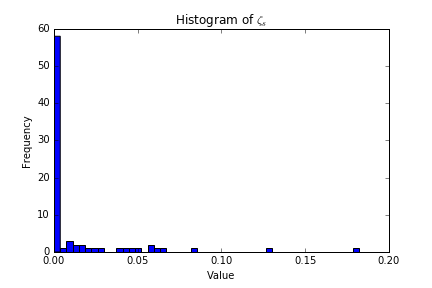
\includegraphics[scale=.8]{code/images/zeta_s_hist}
\caption{Histogram for the distribution of $\zeta_s$.}
\end{figure}

\begin{figure}[h!]
\centering
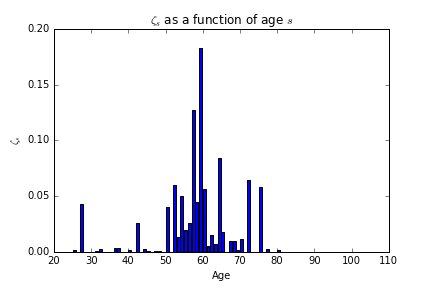
\includegraphics[scale=.8]{code/images/zeta_func}
\caption{$\zeta_s$ plotted as a histogram.}
\end{figure}

\begin{figure}[h!]
\centering
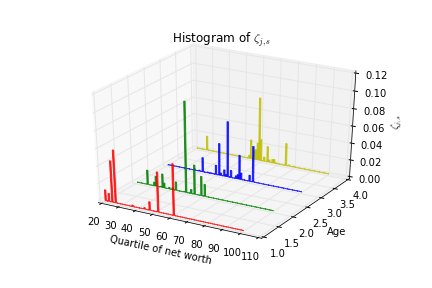
\includegraphics[scale=.8]{code/images/zeta_js_hist}
\caption{$\zeta_{j,s}$ plotted as a histogram.}
\end{figure}

\begin{figure}[h!]
\centering
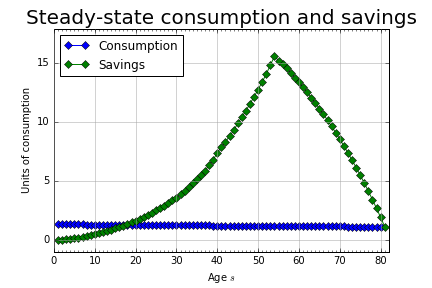
\includegraphics[scale=.8]{code/images/SS_bc}
\caption{Distribution of steady state consumption and savings by age.}
\end{figure}

\end{document}







 	